%============================================================================%
% Antoine Gé́ré (gereantoine@gmail.com).
%============================================================================%


% LaTeX environment used : Kile, available at : http://kile.sourceforge.net/
%
% Package used : available at http://www.ctan.org/
%
% The comprehensive latex symbole list : available at http://www.ctan.org/tex-archive/info/symbols/comprehensive/
% and Detexif, an attempt to simplify to search in the list : available at http://detexify.kirelabs.org/classify.html
%
% Bibliography done with Zotero , available at : https://www.zotero.org/
% Bibtex style ????? .


%----------------------------------------------------------------------------%

\documentclass[10pt]{book}

%----------------------------------------------------------------------------%

%a
\usepackage{amscd}
\usepackage{amsmath}
\usepackage{amsfonts}
\usepackage{amssymb}
\usepackage{amsxtra}
\usepackage{array} 
%b
\usepackage[english]{babel}
%c
\usepackage{cite}
\usepackage{color}
%e
\usepackage{enumitem}
%f
\usepackage{fancyhdr}
\usepackage{filecontents}
\usepackage[T1]{fontenc}
%g
\usepackage{geometry}
%h
\usepackage{hyperref}
%i
\usepackage[totoc]{idxlayout}
\usepackage[utf8]{inputenc}
%m
\usepackage{makeidx}
%n
\usepackage[thmmarks]{ntheorem}
%q
\usepackage[sfdefault]{quattrocento}
%t
\usepackage{tikz}
%u
\usepackage{upgreek}
%w
\usepackage{wrapfig}

%----------------------------------------------------------------------------%

\begin{filecontents}{biblio.bib}
%
%
@article{Gere:2015qsa,
      author         = "Géré, Antoine and Hack, Thomas-Paul and Pinamonti, Nicola",
      title          = "An analytic regularisation scheme on curved spacetimes with applications to cosmological spacetimes",
      year           = "2015",
      eprint         = "1505.00286",
      archivePrefix  = "arXiv",
      primaryClass   = "math-ph",
      SLACcitation   = "%%CITATION = ARXIV:1505.00286;%%",
}
%
%
@article{Duetsch:2002yp,
      author         = "Duetsch, Michael and Fredenhagen, Klaus",
      title          = "The Master Ward Identity and generalized Schwinger-Dyson equation in classical field theory",
      journal        = "Commun.Math.Phys.",
      volume         = "243",
      pages          = "275-314",
      doi            = "10.1007/s00220-003-0968-4",
      year           = "2003",
      eprint         = "hep-th/0211242",
      archivePrefix  = "arXiv",
      primaryClass   = "hep-th",
      reportNumber   = "DESY-02-211",
      SLACcitation   = "%%CITATION = HEP-TH/0211242;%%",
}
%
%
@article{Brunetti:2012ar,
      author         = "Brunetti, Romeo and Fredenhagen, Klaus and Ribeiro, Pedro
                        Lauridsen",
      title          = "Algebraic Structure of Classical Field Theory I: Kinematics and Linearized Dynamics for Real Scalar Fields",
      year           = "2012",
      eprint         = "1209.2148",
      archivePrefix  = "arXiv",
      primaryClass   = "math-ph",
      SLACcitation   = "%%CITATION = ARXIV:1209.2148;%%",
}
%
%
@article{Bar:2007zz,
      author         = "Bar, Christian and Ginoux, Nicolas and Pfaffle, Frank",
      title          = "Wave equations on Lorenzian manifolds and quantization",
      journal        = "ESI Lectures in Mathematical Physics. Zürich: European Mathematical Society",
      pages          = "1-199",
      doi            = "10.4171/037",
      year           = "2007",
      eprint         = "0806.1036",
      archivePrefix  = "arXiv",
      primaryClass   = "math.DG",
      SLACcitation   = "%%CITATION = INSPIRE-773698;%%",
}
%
%
@book{waldGR,
      author         = "Wald, R.M.",
      title          = "General Relativity",
      publisher      = "University of Chicago Press",
      year           = "2010",
      isbn           = "9780226870373",
      url            =  "http://www.worldcat.org/isbn/0226870332",
}
%
%
@article{Khavkine:2014mta,
      author         = "Khavkine, Igor and Moretti, Valter",
      title          = "Algebraic QFT in Curved Spacetime and quasifree Hadamard states: an introduction",
      year           = "2014",
      eprint         = "1412.5945",
      archivePrefix  = "arXiv",
      primaryClass   = "math-ph",
      SLACcitation   = "%%CITATION = ARXIV:1412.5945;%%",
}
%
%
@article{Hack:2010iw,
      author         = "Hack, Thomas-Paul",
      title          = "On the Backreaction of Scalar and Spinor Quantum Fields in Curved Spacetimes",
      year           = "2010",
      eprint         = "1008.1776",
      archivePrefix  = "arXiv",
      primaryClass   = "gr-qc",
      reportNumber   = "DESY-THESIS-2010-042",
      SLACcitation   = "%%CITATION = ARXIV:1008.1776;%%",
}
%
%
\end{filecontents}

%----------------------------------------------------------------------------%

\geometry{
a4paper,
left=20mm,
right=20mm,
top=20mm,
bottom=20mm,
}

%----------------------------------------------------------------------------%

\setlength\parindent{0pt}

%----------------------------------------------------------------------------%

\pdfoptionpdfminorversion=6

%----------------------------------------------------------------------------%

\makeindex

%----------------------------------------------------------------------------%

\renewcommand{\headrulewidth}{0pt}
\renewcommand{\footrulewidth}{0pt}

\setlength{\headheight}{22pt} 

\pagestyle{fancy}
%
\renewcommand{\chaptermark}[1]{ \markboth{#1}{} }
\renewcommand{\sectionmark}[1]{ \markright{#1} }
%
\fancyhf{}
\fancyhead[LE,RO]{\thepage}
\fancyhead[RE,CE]{}
\fancyhead[LO,CO]{}

\fancypagestyle{plain}{ %
\fancyhf{}
}

%----------------------------------------------------------------------------%

\newcommand{\supp}{\mathsf{supp}}
\newcommand{\WF}{\mathsf{WF}}
\newcommand{\id}{\mathsf{id}}

\newcommand{\abs}[1]{\left|#1\right|}
\newcommand{\sm}[1]{\left\langle#1\right\rangle}

\renewcommand{\det}{\mathsf{det}}

%----------------------------------------------------------------------------%

\newcommand{\Acal}{\mathcal{A}}
\newcommand{\Bcal}{\mathcal{B}}
\newcommand{\Ccal}{\mathcal{C}}
\newcommand{\Dcal}{\mathcal{D}}
\newcommand{\Ecal}{\mathcal{E}}
\newcommand{\Fcal}{\mathcal{F}}
\newcommand{\Gcal}{\mathcal{G}}
\newcommand{\Hcal}{\mathcal{H}}
\newcommand{\Ical}{\mathcal{I}}
\newcommand{\Jcal}{\mathcal{J}}
\newcommand{\Kcal}{\mathcal{K}}
\newcommand{\Lcal}{\mathcal{L}}
\newcommand{\Mcal}{\mathcal{M}}
\newcommand{\Ncal}{\mathcal{N}}
\newcommand{\Ocal}{\mathcal{O}}
\newcommand{\Pcal}{\mathcal{P}}
\newcommand{\Qcal}{\mathcal{Q}}
\newcommand{\Rcal}{\mathcal{R}}
\newcommand{\Scal}{\mathcal{S}}
\newcommand{\Tcal}{\mathcal{T}}
\newcommand{\Ucal}{\mathcal{U}}
\newcommand{\Vcal}{\mathcal{V}}
\newcommand{\Wcal}{\mathcal{W}}
\newcommand{\Xcal}{\mathcal{X}}
\newcommand{\Ycal}{\mathcal{Y}}
\newcommand{\Zcal}{\mathcal{Z}}

%----------------------------------------------------------------------------%

\newcommand{\Abb}{\mathbb{A}}
\newcommand{\Bmbb}{\mathbb{B}}
\newcommand{\Cbb}{\mathbb{C}}
\newcommand{\Dbb}{\mathbb{D}}
\newcommand{\Ebb}{\mathbb{E}}
\newcommand{\Fbb}{\mathbb{F}}
\newcommand{\Gbb}{\mathbb{G}}
\newcommand{\Hbb}{\mathbb{H}}
\newcommand{\Ibb}{\mathbb{I}}
\newcommand{\Jbb}{\mathbb{J}}
\newcommand{\Kbb}{\mathbb{K}}
\newcommand{\Lbb}{\mathbb{L}}
\newcommand{\Mbb}{\mathbb{M}}
\newcommand{\Nbb}{\mathbb{N}}
\newcommand{\Obb}{\mathbb{O}}
\newcommand{\Pbb}{\mathbb{P}}
\newcommand{\Qbb}{\mathbb{Q}}
\newcommand{\Rbb}{\mathbb{R}}
\newcommand{\Sbb}{\mathbb{S}}
\newcommand{\Tbb}{\mathbb{T}}
\newcommand{\Ubb}{\mathbb{U}}
\newcommand{\Vbb}{\mathbb{V}}
\newcommand{\Wbb}{\mathbb{W}}
\newcommand{\Xbb}{\mathbb{X}}
\newcommand{\Ybb}{\mathbb{Y}}
\newcommand{\Zbb}{\mathbb{Z}}

%----------------------------------------------------------------------------%

\newcommand{\Arak}{\mathfrak{A}}
\newcommand{\Brak}{\mathfrak{B}}
\newcommand{\Crak}{\mathfrak{C}}
\newcommand{\Drak}{\mathfrak{D}}
\newcommand{\Erak}{\mathfrak{E}}
\newcommand{\Frak}{\mathfrak{F}}
\newcommand{\Grak}{\mathfrak{G}}
\newcommand{\Hrak}{\mathfrak{H}}
\newcommand{\Irak}{\mathfrak{I}}
\newcommand{\Jrak}{\mathfrak{J}}
\newcommand{\Krak}{\mathfrak{K}}
\newcommand{\Lrak}{\mathfrak{L}}
\newcommand{\Mrak}{\mathfrak{M}}
\newcommand{\Nrak}{\mathfrak{N}}
\newcommand{\Orak}{\mathfrak{O}}
\newcommand{\Prak}{\mathfrak{P}}
\newcommand{\Qrak}{\mathfrak{Q}}
\newcommand{\Rrak}{\mathfrak{R}}
\newcommand{\Srak}{\mathfrak{S}}
\newcommand{\Trak}{\mathfrak{T}}
\newcommand{\Urak}{\mathfrak{U}}
\newcommand{\Vrak}{\mathfrak{V}}
\newcommand{\Wrak}{\mathfrak{W}}
\newcommand{\Xrak}{\mathfrak{X}}
\newcommand{\Yrak}{\mathfrak{Y}}
\newcommand{\Zrak}{\mathfrak{Z}}

%----------------------------------------------------------------------------%

\newcommand{\Asf}{\mathsf{A}}
\newcommand{\Bsf}{\mathsf{B}}
\newcommand{\Csf}{\mathsf{C}}
\newcommand{\Dsf}{\mathsf{D}}
\newcommand{\Esf}{\mathsf{E}}
\newcommand{\Fsf}{\mathsf{F}}
\newcommand{\Gsf}{\mathsf{G}}
\newcommand{\Hsf}{\mathsf{H}}
\newcommand{\Isf}{\mathsf{I}}
\newcommand{\Jsf}{\mathsf{J}}
\newcommand{\Ksf}{\mathsf{K}}
\newcommand{\Lsf}{\mathsf{L}}
\newcommand{\Msf}{\mathsf{M}}
\newcommand{\Nsf}{\mathsf{N}}
\newcommand{\Osf}{\mathsf{O}}
\newcommand{\Psf}{\mathsf{P}}
\newcommand{\Qsf}{\mathsf{Q}}
\newcommand{\Rsf}{\mathsf{R}}
\newcommand{\Ssf}{\mathsf{S}}
\newcommand{\Tsf}{\mathsf{T}}
\newcommand{\Usf}{\mathsf{U}}
\newcommand{\Vsf}{\mathsf{V}}
\newcommand{\Wsf}{\mathsf{W}}
\newcommand{\Xsf}{\mathsf{X}}
\newcommand{\Ysf}{\mathsf{Y}}
\newcommand{\Zsf}{\mathsf{Z}}

\newcommand{\asf}{\mathsf{a}}
\newcommand{\bsf}{\mathsf{b}}
\newcommand{\csf}{\mathsf{c}}
\newcommand{\dsf}{\mathsf{d}}
\newcommand{\esf}{\mathsf{e}}
\newcommand{\fsf}{\mathsf{f}}
\newcommand{\gsf}{\mathsf{g}}
\newcommand{\hsf}{\mathsf{h}}
\newcommand{\isf}{\mathsf{i}}
\newcommand{\jsf}{\mathsf{j}}
\newcommand{\ksf}{\mathsf{k}}
\newcommand{\lsf}{\mathsf{l}}
\newcommand{\msf}{\mathsf{m}}
\newcommand{\nsf}{\mathsf{n}}
\newcommand{\osf}{\mathsf{o}}
\newcommand{\psf}{\mathsf{p}}
\newcommand{\qsf}{\mathsf{q}}
\newcommand{\rsf}{\mathsf{r}}
\newcommand{\ssf}{\mathsf{s}}
\newcommand{\tsf}{\mathsf{t}}
\newcommand{\usf}{\mathsf{u}}
\newcommand{\vsf}{\mathsf{v}}
\newcommand{\wsf}{\mathsf{w}}
\newcommand{\xsf}{\mathsf{x}}
\newcommand{\ysf}{\mathsf{y}}
\newcommand{\zsf}{\mathsf{z}}

%----------------------------------------------------------------------------%

\newcommand*{\makepagetitle}{%
%
{\raggedright% 
%
%
%
%
\thispagestyle{empty}%
%
\vspace*{50pt}
%
{\LARGE Antoine Géré}\\% 
%
\vspace*{120pt}%
%
{\Huge\bfseries Algebraic and Noncommutative \\[8pt] approaches to Quantum Field Theory}\\[\baselineskip]%
%
\vspace*{60pt}%
%
{\LARGE Ph.D. thesis}\\[\baselineskip]% 
%
\vspace*{60pt}%
%
{\LARGE Dipartimento di Matematica}\\[\baselineskip]% 
%
\vspace*{1pt}
%
{\LARGE Università degli Studi di Genova}\\[\baselineskip]% 
%
\vfill% 
%
%
%
%
\newpage%
%
\thispagestyle{empty}%
%
%\begin{figure}[h]%

\includegraphics[scale=1]{unige.pdf}
% unige.pdf: 29x39 pixel, 72dpi, 1.02x1.38 cm, bb=0 0 29 39
%\end{figure}
%
\ \vfill%
%
%
\textbf{Algebraic and Noncommutative approaches to Quantum Field Theory} \\[2pt]
Ph.D. thesis submitted by \href{mailto:gere@dima.unige.it}{Antoine Géré} \\[1pt]
\href{(blablabla)}{Genova}, ???? 2016 \\[10pt]
%
\href{(blablabla)}{Dipartimento di Matematica} \\[1pt]
\href{(blablabla)}{Università degli Studi di Genova} \\[10pt]
%
Supervisor: \href{mailto:pinamont@dima.unige.it}{Prof. Dr. Nicola Pinamonti} \\[1pt]
Examiner: ????
%
%
%
%
%
}%
%
}%

%----------------------------------------------------------------------------%

\theoremclass{LaTeX}
\theoremstyle{break}
\theoremheaderfont{\normalfont\bfseries}
\theorembodyfont{\normalfont}
\theoremseparator{}
\theoremsymbol{\ensuremath{\blacktriangleright}}
\newtheorem{theorem}{Theorem}
\newtheorem{proposition}{Proposition}
\newtheorem{lemma}{Lemma}
\newtheorem{corollary}{Corollary}
\theoremsymbol{\ensuremath{\blacklozenge}}
\newtheorem{example}{Example}
\newtheorem{remark}{Remark}
\newtheorem{definition}{Definition}
\theoremsymbol{\ensuremath{\blacksquare}}
\newtheorem{proof}{Proof}
\qedsymbol{\ensuremath{_\blacksquare}}

%----------------------------------------------------------------------------%

\definecolor{hypercolor}{rgb}{0.1,0.2,0.6}

\hypersetup{     
 unicode=false,      
 pdftoolbar=true,    
 pdfmenubar=true,    
 pdffitwindow=true,  
 pdfstartview={FitH},
 pdftitle={PhD thesis},    
 pdfauthor={Antoine Géré},     
 pdfsubject={Mathematical Physics},
 pdfcreator={LaTeX},  
 pdfproducer={pdfTex},
 pdfkeywords={Algebraic Quantum Field Theory; Noncommutative Field Theory.},  
 pdfnewwindow=true,  
 colorlinks=true, 
 linkcolor=hypercolor, 
 urlcolor=hypercolor, 
 citecolor=hypercolor,
 filecolor=hypercolor,         
}

%============================================================================%
\begin{document}
%============================================================================%

\pagenumbering{Roman}

\makepagetitle

\newpage

%----------------------------------------------------------------------------%

\ \vfill

\begin{flushright}
to (blablabla) 
\end{flushright}

\vfill

%----------------------------------------------------------------------------%

\newpage

\ \vfill

\begin{flushright}
citation
\end{flushright}

\vfill

%----------------------------------------------------------------------------%

\newpage

\vspace*{100pt}

\thispagestyle{empty}

\section*{Abstract}

(blablabla)

%----------------------------------------------------------------------------%

\tableofcontents

%----------------------------------------------------------------------------%

\part*{Introduction}
\addcontentsline{toc}{part}{Introduction}
\pagenumbering{arabic}

%----------------------------------------------------------------------------%

(blablabla)

%----------------------------------------------------------------------------%
\part{Algebraic approach to quantum field theory}
%----------------------------------------------------------------------------%

%----------------------------------------------------------------------------%
\chapter{Spacetime}
%----------------------------------------------------------------------------%


The starting block for a physical theory is the notion of spacetime. Looked at space and time as an unique entity has been an important turning point in the understanding of ``the laws of nature''. Newton's physics treated them separately, but at the beginning of the last century Einstein introduced a completely new point of view of these two entities. In his theory of gravitation, the physical background (i.e. the spacetime) is an ``active actor''. Indeed gravitation roughly speaking can be viewed as a deformation of the spacetime. Therefore we shall introduce the notion of spacetime starting from the very beginning.


%----------------------------------------------------------------------------%
\section{From topology to manifold}
%----------------------------------------------------------------------------%

The most fundamental way to define a space is to use the notion of topology. It is concerned with the intrinsec properties of spaces.

\begin{definition}[Topological space] \index{topological space}
Let $\Xsf$ be a set. A topology on $\Xsf$ is a collection $\Tcal$ of subsets satisfying the three following axioms,%
%
\begin{itemize}
\item \textbf{conventions on empty set} : $\emptyset , \ \Xsf \in \Tcal$ ;
\item \textbf{arbitrary union} : $U_i \in \Tcal \mbox{ for } i \in I \Longrightarrow \bigcup_{i\in I} U_i \in \Tcal$, where $I$ is an arbitrary index set ;
\item \textbf{finite intersection} : $U_1 , \dots , U_n \in \Tcal \Longrightarrow U_1 \cap \dots \cap U_n \in \Tcal$ .
\end{itemize}
%
\end{definition}


The pair $(\Xsf,\Tcal)$ is called a topological space. The element of $\Tcal$ are the open sets of $\Xsf$. We shall often omit to precise the topology $\Tcal$, and simply say that $\Xsf$ is a topological space. It is still general, nonetheless it already characterizes maps between different topological spaces.\par%


\begin{definition}[Continous maps and homeomorphism]
Let $\Xsf$ and $\Ysf$ be topological spaces. We consider a map $f : \Xsf \to \Ysf$. We say
%
\begin{itemize}
\item $f$ is \textbf{continous} if $f^{-1}(U) \subset X$ is open for every open $U \subset\Ysf$ ;
\item $f$ is a \textbf{homeomorphism} if $f$ is bijective and both $f$ and $f^{-1}$ are continous.
\end{itemize}
%
\end{definition}


In the purpose of implementing ``some physics'' on these spaces we need more than only the topological structure. A first step is to give meaning of notion of distance, also called metric.


\begin{definition}[Metric]
Let $\Xcal$ be a set. A metric on $\Xcal$ is a map $g : \Xcal \times \Xcal \to \Rbb_+$ such that for all $x, y, z \in \Xcal$,%
%
\begin{itemize}
\item \textbf{separation} : $g(x,y) = 0 \Leftrightarrow x=y$ ; 
\item \textbf{symetry} : $g(x,y) = g(y,x)$ ;
\item \textbf{triangle inequality} : $g(x,y) \leq g(x,z) + g(z,y)$ .
\end{itemize}
%
\end{definition}


A set $\Xcal$ endowed with a metric $g$ is called a metric space, and denoted $(\Xcal,g)$. We can show that a metric space is also a topological space for which the topology is induced by the metric. Let us detail this in the following lemma.


\begin{lemma}[Topological metric space]
Every metric space $(\Xcal,g)$ is also a topological space for which the topology is induced by the collection of open sets in $\Xcal(=\Xsf)$. We denote it by $(\Xsf,\Tcal_g)$.
\end{lemma}


\begin{proof}
%%TODO
Decide if i show the proof or not.
%We shall consider the following collection of open subsets in $\Xcal$.
%
%\begin{equation*}
%\Tcal_g = \left\{ B_i \right\}_{i \in I} = \left\{B_i = B(x_i,\epsilon) , i \in I \ \bigg| \ \forall x_i \in \Xcal , \ \exists \epsilon > 0, \ B(x_i,\epsilon) = \left\{ y \in \Xcal , g(x_i,y) < \epsilon \right\} \subset \Xcal \right\}
%\end{equation*}
%
%First observation is that $\emptyset$ and $\Xcal$ are open and contained in $\Tcal_g$. Indeed there are no points in the empty set, therefore it is true that $x \in \emptyset$ whenever $g(x,e) < 1$, $\forall e \in \emptyset$, and conservely every points $x$ belongs to $\Xcal$, therefore it is also true that $x \in \Xcal$ whenever $g(x,e) < 1$,  $\forall e \in \Xcal$.\par%
%
%Second observation is because $B_i$ is open $\forall i \in I$, then $\bigcup_{i\in I} B_i$ is open. Indeed if $e \in \bigcup_{i\in I} B_i$, then we can find a particular $i_1 \in I$ with $e \in V_{i_1}$. Since $B_{i_1}$ is open we can find $\epsilon > 0$ such that $x \in B_{i_1}$ whenever $g(x,e) < \epsilon$. And since $B_{i_1} \subseteq \bigcup_{i\in I} U_i$ we have $x \in \bigcup_{i\in I} B_i$ whenever $g(x,e) <e$. Thus $\bigcup_{i\in I} B_i$ is open and contained in $\Tcal_g$.\par%
%
%Third and last observation is that if $B_j$ is open $\forall j \in J$, then $\bigcap_{j\in J} B_j$ is open. Indeed if $e \in \bigcap_{j \in J} B_j$, then $e \in B_j$, $\forall j \in J$. Since $B_j$ is open we can find a $\epsilon_j > 0$ such that $x \in B_j$ whenever $g(x,e) < \epsilon_j$. We set $\epsilon = min_{j\in J} \epsilon_j (>0)$, then we have $x \in B_j$ whenever $d(x,e) < \epsilon$, $\forall j \in J$. Thus $x \in \bigcap_{j\in J} B_j$ whenever $d(x,e) < \epsilon$, and therefore $\bigcap_{j\in J} B_j$ is open and contained $\Tcal_g$.\par%
\end{proof}


Let us give some generic definition which shall appear to be useful later on. $\Xsf$ shall always denote a topological space with topology $\Tcal$, and $\Zsf$ a subspace of $\Xsf$.%


\begin{enumerate}
%
\item $\overline{\Zsf}$, the \textbf{closure} of $\Zsf \subset \Xsf$, is the intersection of all closed sets\footnote{A set $\Csf \subset \Xsf$ is \textbf{closed} if $\Xsf \backslash \Csf$ is open.} containing $\Zsf$.% 
%
\item $\Zsf$ is \textbf{dense} in $\Xsf$ if $\overline{\Zsf} = \Xsf$.%
%
\item $\Bcal \subset \Tcal$ is a \textbf{topological basis} if every elements in $\Tcal$ can be written as the union of elements of the bais $\Bcal$.%
%
\item $\Xsf$ is \textbf{second countable} if it has a countable\footnote{A set is said to be \textbf{countable} if there exists a one to one correspondence between the set considered and the set of natural numbers.} topological basis.%
%
\item $\Xsf$ is \textbf{separable} if there exists a dense and countable subset.%
%
\item $\Ksf \subset \Xsf$ is \textbf{compact} if any covering of it admit a finite subcovering.%
%
\item $\Xsf$ is \textbf{locally compact} if every point in $\Xsf$ admit a neighborhood which has compact closure.%
%
\item $\Xsf$ is \textbf{connected} if it cannot be written as a disjoint union of two nonempty open subsets.%
%
\item $\Xsf$ is \textbf{Hausdorff} if every pair of points have disjoint neighborhood.%
%
\item $\Xsf$ is \textbf{paracompact} if every open cover has a refinement covering that is locally finite\footnote{$\left\{\Usf_\alpha\right\}$, a cover of $\Xsf$, is \textbf{locally finitte} if every points in $\Xsf$ has a neighborhood which has a nonempty intersection with a finite numbers of $\Usf_\alpha$.}.%
%
\item $\Xsf$ is said to be \textbf{metrizable} if there is a metric on $\Xsf$ for which the induced topology is $\Tcal$.
%
\end{enumerate}


We shall later one consider only Hausdorff topological spaces which shall also be metric spaces. Therefore it is interesting to consider the following lemma.


\begin{lemma}[Hausdorff metric space]
Every metric space is Hausdorff. 
\end{lemma}


\begin{proof}
%%TODO
Decide if i show the proof or not.
%Let $x$ and $y$ be two points of a topological space $\Xsf$, and $U_x$ (respectively $U_y$) a neighborhood of $x$ (respectively of $y$). We set the radius of the two neighborhoods as $g(x,y)/2$. We suppose now that $U_x$ and $U_y$ are not disjoint, then we can always find a point $z$ which belong in both neighborhood. Using the triangle inequality an the fact that $g(x,z) < g(x,y)/2$ and $g(x,z) < g(x,y)/2$, we get that $g(x,y) < g(x,y)$ which is a contradiction. Therefore the two neighborhoods are disjoint and every metric space is Hausdorff.
\end{proof}


For later puposes we give an equivalence lemma between Hausdorff and secound countable, and metrizable and separable spaces.

\begin{lemma}
Let $\Xsf$ be a topological spce of dimension $n$ in which all points admit a neighborhood homeomorphic to an open set in $\Rbb^n$. Then the following two properties are equivalent
%
\begin{enumerate}
\item $\Xsf$ is Hausdorff and second countable ;
\item $\Xsf$ is metrizable and separable.
\end{enumerate}
%
\end{lemma}


\begin{proof}
%%TODO
Decide if i show the proof or not.
\end{proof}


We have now enough background to introduce the fundamental notion of manifold. We start with topological manifolds and will implement differential structure in the next section.


\begin{definition}[Topological manifold]
A topological manifold $\Mcal$ of dimension $n$ is a Hausdorff and second countable topological space in which every points admit an open neighborhood homeomorphic to a subset of $\Rbb^n$.
\end{definition}

Due to the previous lemma, instead of asking to $\Mcal$ to be Hausdorff and second countable, we can ask to be separable and metrizable. But these properties are global, what is important is that $\Mcal$ admit locally the same topological properties as $\Rbb^n$.\par%


\bigskip


An important tool to pass from a local to a global point of view is the \textbf{partition of unity} of $\Xsf$. It is a collection of continous maps $(\phi_i)_{i \in I}$, $\phi_i : \Xsf \to [0,1]$, such that the collection of their supports is locally finite, and that $\sum_{i\in I} \phi_i = 1$. We call, $(\phi_i)_{i \in I}$, partition of unity subordinate to an open cover $U=(U_i)_{i \in I}$, if for all $i \in I$, the support of $\phi_i$ is contained in $U_i$.


\begin{lemma}
A topological manifold $\Mcal$ is paracompact and admit a partition of unity subordinate to every open cover of $\Mcal$.
\end{lemma}


\begin{proof}
%%TODO
Decide if i show the proof or not.
\end{proof}


%----------------------------------------------------------------------------%
\section{Lorentzian manifold}
%----------------------------------------------------------------------------%

We gave the definition of a topological manifold in the previous section. We want now to implement differential structure in order to be able to define what is a smooth manifold.

\bigskip

Let $\Mcal$ be a topological manifold of dimension $n$. We would like to be able to ``localize'' points on a manifold, it is done via the notion of a chart. A chart on $\Mcal$ is a pair $(U,\phi)$, where $U$ is an open subset on $\Mcal$ and $\phi$ is a homeomorphism from $U$ to an open subset $\phi(U) \subset \Rbb^n$. We call $U$ a coordinate neighborhood, $\phi$ a coordinate maps, and the component functions of $\phi$ local coordinates on $U$.

\begin{figure}[h]
\begin{center}
\begin{tikzpicture}[thick,scale=0.7] 
%
%
\draw[color=black] (0,0) to [out=50,in=190] (6,3);
\draw[color=black] (6,3) to [out=10,in=90] (10,0);
\draw[color=black] (10,0) to [out=170,in=30] (3,-3);
\draw[color=black] (3,-3) to [out=90,in=10] (0,0);
%
\filldraw (6.5,2.2) circle (0pt) node[above] {$\Mcal$}; 
%
\def\firstellipse{(4,0.5) ellipse (1.6 and 0.6)};
\def\secondellipse{(6,1) ellipse (1.6 and 0.6)};
\draw[color=black] \firstellipse \secondellipse;
%
\filldraw (3.5,1) circle (0pt) node[above] {$U$}; 
\filldraw (8,01) circle (0pt) node[above] {$V$}; 
%
\begin{scope}
\clip \firstellipse;
\fill[green] \secondellipse;
\end{scope}
%
%
\draw[dashed] (-3,-7) -- (-1,-5) -- (3,-5) -- (1,-7) -- (-3,-7);
\filldraw (1,-7) circle (0pt) node[below] {$\Rbb^n$}; 
\draw[color=black] (0,-6) ellipse (1.6 and 0.6);
\filldraw (-1.9,-7.1) circle (0pt) node[above] {$\phi(U)$}; 
%
%
\draw[dashed] (7,-7) -- (9,-5) -- (13,-5) -- (11,-7) -- (7,-7);
\filldraw (11,-7) circle (0pt) node[below] {$\Rbb^n$}; 
\draw[color=black] (10,-6) ellipse (1.6 and 0.6); 
\filldraw (8.2,-7.1) circle (0pt) node[above] {$\psi(V)$};
%
%
\draw[->,dashed,color=black] (1.5,-1.5) -- (0.5,-4.5);
\filldraw (1,-3.2) circle (0pt) node[right] {$\phi$}; 
%
%
\draw[->,dashed,color=black] (7.5,-1) -- (9.5,-4.5);
\filldraw (8.9,-3.2) circle (0pt) node[right] {$\psi$}; 
%
%
\draw[->,dashed,color=black] (3,-6) -- (7,-6);
\filldraw (5,-6) circle (0pt) node[above] {$\psi \circ \phi^{-1}$}; 
%
%
\end{tikzpicture}
\end{center}
\caption{Charts and transition function.}
\end{figure}


In order to make sense of smooth manifold, we need to implement an additional notion to the topology. Let $(\phi,U)$ and $(\psi,V)$ be two charts on $\Mcal$ such that $U \cap V \neq \emptyset$. We call transition map, the application
%
\begin{equation*}
\psi \circ \phi^{-1} \ : \ \phi(U \cap V) \subset \Rbb^n \ \to \ \psi(U \cap V) \subset \Rbb^n \ .
\end{equation*}
%
It is a homeomorphism. We say $(\phi,U)$ and $(\psi,V)$ are smoothly compatible if $U \cap V = \emptyset$ or the transition map $\phi^{-1} \circ \psi$ is a diffeomorphism, i.e. bijective with smooth inverse.


\bigskip


We call an atlas of $\Mcal$ a set of chart $\left\{ (U, \phi) \right\}$ which covers $\Mcal$. An atlas $\Acal$ is called smooth if any two charts in $\Acal$ are smoothly compatible. A smooth atlas $\Acal$ is called maximal if it is not contained in any stricly larger smooth atlas. We now can give the definition of a smooth manifold.


\begin{definition}[Smooth manifold]
$\Mcal$ is a smmooth manifold if $\Mcal$ is a topological manifold with a smooth maximal atlas $\left\{(U,\phi)\right\}$.
\end{definition}

Let us define the notion of a smooth (compactly supported) function.

\begin{definition}[Smooth - compactly supported - function]
A function $f : \Mcal \to \Rbb$ is said to be smooth if and only if $f \circ \phi^{-1} : \phi(U) \subset \Rbb^n \to f(U) \subset \Rbb$ is smooth for each coordinate chart in the atlas.\par%
A function $f : \Mcal \to \Rbb$ is said to be compactly supported if the support of $f : \Mcal \to \Rbb$ (i.e. the closure of the set where $f$ does not vanish) is compact. 
\end{definition}


For now on $\Mcal$ shall be understood as a smooth manifold. The set of all smooth function on $\Mcal$ is denoted by $\Ecal(\Mcal)$. And the one for smooth compactly supported functions on $\Mcal$ is denoted by $\Dcal(\Mcal)$. 


\begin{figure}[ht]
\begin{center}
\begin{tikzpicture}[thick,scale=0.7] 
\draw[color=black] (0,0) to [out=50,in=190] (6,3);
\draw[color=black] (6,3) to [out=10,in=90] (10,0);
\draw[color=black] (10,0) to [out=170,in=30] (3,-3);
\draw[color=black] (3,-3) to [out=90,in=10] (0,0);
\draw[color=black] (5.2,1) ellipse (2 and 1);
\filldraw (10,0) circle (0pt) node[right] {$\Mcal$}; 
\filldraw (3,0) circle (0pt) node[above] {$U$}; 
%
\draw[->,color=black,dashed] (5,-2.5) -- (5,-4.5);
\filldraw (5,-3.5) circle (0pt) node[right] {$\phi$}; 
%
\draw[dashed] (1,-7) -- (3,-5) -- (9,-5) -- (7,-7) -- (1,-7);
\draw[color=black] (5,-6) ellipse (1.6 and 0.6);
\filldraw (9,-5) circle (0pt) node[right] {$\Rbb^n$}; 
\filldraw (3,-7) circle (0pt) node[above] {$\phi(U)$}; 
%
\draw[->,color=black,dashed] (5,-7.5) -- (5,-9.5);
\filldraw (5,-8.5) circle (0pt) node[right] {$f \circ \phi^{-1}$}; 
%
\draw[line width=0.8mm,color=black] (3,-10) -- (7,-10);
\draw[color=black] (0,-10) -- (10,-10);
\filldraw (10,-10) circle (0pt) node[right] {$\Rbb$};
\filldraw (3,-10) circle (0pt) node[above] {$f(U)$}; 
%
\draw[->,color=black,dashed] (0,-0.5) -- (0,-9.5);
\filldraw (0,-4.5) circle (0pt) node[right] {$f$}; 
%
\end{tikzpicture}
\end{center}
\caption{Real valued smooth function.}
\end{figure}

\begin{definition}[Smooth map]
A map $f : \Mcal \to \Ncal$ between two smooth manifolds is said to be smooth if there are two $(U,\phi)$ and $(V,\psi)$ on $\Mcal$ and $\Ncal$ respectively, such that the transition function $\psi \circ f \circ \phi^{-1}$ is  smooth.
\end{definition}

We notice that in particular if the two manifolds are of the same dimension then $f$ is said to be a diffeomorphism.

\begin{figure}[ht]
\begin{center}
\begin{tikzpicture}[thick,scale=0.6] 
\draw[color=black] (0,0) to [out=50,in=190] (6,3);
\draw[color=black] (6,3) to [out=10,in=90] (10,0);
\draw[color=black] (10,0) to [out=170,in=30] (3,-3);
\draw[color=black] (3,-3) to [out=90,in=10] (0,0);
\draw[color=black] (5.2,1) ellipse (2 and 1);
\filldraw (10,0) circle (0pt) node[right] {$\Mcal$}; 
\filldraw (3,0) circle (0pt) node[above] {$U$};
\filldraw (5,1) circle (2pt) node[above] {$x$};
%
\draw[color=black] (15,0) to [out=50,in=190] (21,3);
\draw[color=black] (21,3) to [out=10,in=90] (25,0);
\draw[color=black] (25,0) to [out=170,in=30] (18,-3);
\draw[color=black] (18,-3) to [out=90,in=10] (15,0);
\draw[color=black] (20.2,1) ellipse (2 and 1);
\filldraw (25,0) circle (0pt) node[right] {$\Ncal$}; 
\filldraw (18,0) circle (0pt) node[above] {$V$}; 
\filldraw (20,1) circle (2pt) node[above] {$f(x)$};
%
\draw[->,color=black,dashed] (5,-2.5) -- (5,-4.5);
\filldraw (5,-3.5) circle (0pt) node[right] {$\phi$}; 
%
\draw[dashed] (1,-7) -- (3,-5) -- (9,-5) -- (7,-7) -- (1,-7);
\draw[color=black] (5,-6) ellipse (1.6 and 0.6);
\filldraw (9,-5) circle (0pt) node[right] {$\Rbb^n$}; 
\filldraw (2.5,-7) circle (0pt) node[above] {$\phi(U)$}; 
%
\draw[->,color=black,dashed] (20,-2.5) -- (20,-4.5);
\filldraw (20,-3.5) circle (0pt) node[right] {$\psi$}; 
%
\draw[dashed] (16,-7) -- (18,-5) -- (24,-5) -- (22,-7) -- (16,-7);
\draw[color=black] (20,-6) ellipse (1.6 and 0.6);
\filldraw (24,-5) circle (0pt) node[right] {$\Rbb^n$}; 
\filldraw (17.5,-7) circle (0pt) node[above] {$\psi(V)$}; 
%
\draw[->,color=black,dashed] (9,-6) -- (16,-6);
\filldraw (12.5,-6) circle (0pt) node[above] {$\psi \circ f \circ \phi^{-1}$}; 
%
\draw[->,color=black,dashed] (10,2) -- (16,2);
\filldraw (13,2) circle (0pt) node[above] {$f$}; 
%
\end{tikzpicture}
\end{center}
\caption{Smooth map between manifolds.}
\end{figure}


We define the tangent vectors $V$ as the derivatives of real valued smooth function on $\Mcal$ in a particular direction
%
\begin{equation*}
V_x : \left\{
\begin{array}{cll}
\Ecal(\Mcal) & \to & \Rbb \\
f & \mapsto & \underset{t \to 0}{\lim} \ \frac{1}{t} \left( f(x+tv) - f(x) \right)
\end{array}
\right. \ , \quad \forall x \in \Mcal .
\end{equation*}
%
It is linear and satisfies the Leibniz product rule,
%
\begin{equation*}
V_x(fg) = f(x) V_x(g) + g(x) V(f) .
\end{equation*}
%
The set of all tangent vectors $V_x$ is called the tangent space and denoted by $T_x \Mcal$. A tangent space to a manifold has the same dimension as the given manifold.


\bigskip
%%TODO
ADD FIGURE TO ILLUSTRATE A TANGENT VECTOR / TANGENT SPACE ON A SMOOTH manifold !
\bigskip


Before adding more structure on $T_x M$ we shall introduce the notion of vetor bundle. A smooth real vector bundle is a triple $(E,\Mcal,\pi)$, where $E$ (total space) and $\Mcal$ (base space of dimension $n$) are smooth manifolds and 
%
\begin{equation*}
\pi : E \to \Mcal , 
\end{equation*}
%
is a smooth surjection satisfying
%
\begin{itemize}
\item $E_x = \pi^{-1}(\{x\})$, called the fibre of $E$ at $x\in\Mcal$, is a $n$ dimensional vector space $\forall x \in \Mcal$ ; 
\item $\exists$ an open $U \subseteq \Mcal$, with $x \in U$ and a smooth diffeomorphism $\phi : \pi^{-1}(U) \to U \times E_x$ such that the diagram \ref{fig:vect-bund} commutes.
\end{itemize}
%
\begin{figure}[ht]
\begin{center}
\begin{tikzpicture}[scale=1]
\draw[->,color=black] (0,0) -- (3,0);
\draw[->,color=black] (0,-0.2) -- (1.3,-1.5);
\draw[->,color=black] (3,-0.2) -- (1.7,-1.5);
%
\filldraw (0,0) circle (0pt) node[left] {$\pi^{-1}(U)$};
\filldraw (3,0) circle (0pt) node[right] {$U \times \{ E_x \}$};
\filldraw (1.5,-1.5) circle (0pt) node[below] {$U$};
\end{tikzpicture}
\end{center}
\caption{Vector bundle structure.}
\label{fig:vect-bund}
\end{figure}
%
We call smooth section of a vector bundle a smooth map $s : \Mcal \to E$, such that $\pi \circ s = \id$, the corresponding vector space is denoted $\Gamma(\Mcal)$. We shall later see the importance of the notion of section in physics, it defines the fields.



\bigskip


Then we have two important particular smooth real vector bundles, the ``tangent bundle'' and the ``real line bundle''. Two notion which shall appear to be useful in the following.


\begin{definition}[Tangent/line bundle]
A tangent bundle is the triple $T\Mcal=(T_x\Mcal, \Mcal, \pi_t)$ with $\pi_t : T_x\Mcal \to \Mcal$. Its corresponding section is $v : \Mcal \to T_x\Mcal$.\par
A real line bundle is the triple $(\Rbb, \Mcal, \pi_\ell)$ with $\pi_\ell : \Rbb \to \Mcal$. Its corresponding section is $f : \Mcal \to \Rbb$.
\end{definition}


%We call cotangent space $T^\ast_x\Mcal$ the dual of the tangent space $T_x\Mcal$ at the same point. The cotangent bundle is the triple $T^\ast\Mcal=(T^\ast_x\Mcal, \Mcal, \pi^\ast_t)$ with $\pi^\ast_t : T^\ast_x\Mcal \to \Mcal$.


%Using the different notions previously defined we shall introduce the Lorentzian scalar product, denoted $g_x$. We assign to each point $x \in \Mcal$ a scalar product on the tangent space $T_x\Mcal$,
%
%\begin{equation*}
%g_x : \left\{
%\begin{array}{cll}
%T_x\Mcal & \to & \Rbb \\
%X & \mapsto & - \left(X,X\right) \ ,
%\end{array}
%\right. ,
%\end{equation*}
%
%such that for $\{e_i\}_{i=1,\dots,n}$ a basis of $T_x\Mcal$, we have
%\begin{equation*}
%(e_i,e_j) = 
%\left\{
%\begin{array}{ll}
%-1 & \mbox{ if } \ i=j=1 ; \\
%1  & \mbox{ if } \ i=j=2,\dots,n ; \\
%0  & \mbox{ otherwise} .
%\end{array}
%\right.
%\end{equation*}
%
%The scalar product is a Lorentzian scalar product if for every chart $(U,\phi)$ of $\Mcal$, such that $\phi=(x_1,\dots,x_n)$, the functions
%
%\begin{equation*}
%g_x = g\left(\frac{\partial}{\partial x_i},\frac{\partial}{\partial x_j}\right) = g_{ij} \ : \ T_x\Mcal \to \Rbb
%\end{equation*}
%are smooth\footnote{$\left(\frac{\partial}{\partial x_i}\right)_{i=1,\dots,n}$ is the coordinates of the section of the tangen bundle $T\Mcal$ (vector fields).}


%\bigskip

%We have now enough material to define the so called Lorentzian manifold.


\begin{center}
!!!! LORENTZIAN METRIC !!!!
\end{center}


\begin{definition}[Lorentzian manifold]
$(\Mcal,g)$ is a Lorentzian manifold, where $\Mcal$ is a $n$ dimensional smooth manifold, and g is a Lorentzian metric.
\end{definition}

\begin{center}
!!!! CONNECTTION !!!! \\
!!!! GEODESIC $\to$ SYNGE'S WORLD FUNCTION !!!! \\
!!!! CURVATURE !!!!
\end{center}

%\begin{lemma}[Uniquenes of a maximal atlas]
%Every smooth atlas of $\Mcal$ is contained in an unique maximal smooth atlas.
%\end{lemma}


%----------------------------------------------------------------------------%
\section{Causality}
%----------------------------------------------------------------------------%

\bigskip


\begin{center}
!!!! MODIFY THIS PART !!!!
\end{center}


\bigskip

We are now working with the pair $(\Mcal,g)$ which denotes now a Lorentzian manifold of dimension $n \geq 2$. We associate to each point $x$ of the manifold its conresponding tangent space $T_x\Mcal$. Considering a vector field $v$ on $T_x\Mcal$, we can evaluate its scalar product with itself, using the metric $g$. It divides the tangent space in three different region.
%
\begin{eqnarray*}
g(v,v) &>& 0 , \ \mbox{ then v is called timelike vector}, \\ 
g(v,v) &=& 0 , \ \mbox{ then v is called null vector}, \\ 
g(v,v) &<& 0 , \ \mbox{ then v is called spacelike vector}.
\end{eqnarray*}


The set of all timelike vectors is called the open lightcone 
%
\begin{equation*}
 \Vcal=\Vcal^{+} \ \dot{\cup} \ \Vcal^{-} \ . 
\end{equation*}
%
It is the disjoint union of two connected components, which we refer to as the forward and backward lightcones, 
%
\begin{equation*}
\Vcal^{\pm}=\left\{ x\in\Mcal \ | \ x^{2}>0, \ \pm x^{0}>0 \right\} \ . 
\end{equation*}
%
We denote by $\overline{\Vcal^{\pm}}$ and $\partial\Vcal^{\pm}$ the closure and boundary of these sets, respectively.%


\begin{definition}
A vector $v \in T_x\Mcal$ is \textbf{future} (respectively \textbf{past}) \textbf{directed} if it is timelike or lightlike and $v \in \Vcal^+$ (respectively $v \in \Vcal^-)$. \\[3pt]
A differentiable curve $\gamma(\lambda)$ is said to be 
\begin{description}
\item a \textbf{future} (respectively \textbf{past}) \textbf{directed timelike curve} if at each point $x(\lambda) \in \gamma$ the tangent vector $v$ is a future (respectively past) directed timelike vector ;
\item a \textbf{future} (respectively \textbf{past}) \textbf{directed causal curve} if at each point $x(\lambda) \in \gamma$ the tangent vector $v$ is either a future (respectively past) directed timelike or null vector. 
\end{description} 
\end{definition}

\begin{definition}[Chronological future/past]
The \textbf{chronological future} of $p \in M$, denoted by $I^{+}(p)$ is defined as the sets of events that can be reached by a future directed timelike curve starting from $p$,

\begin{equation*}
I^{+}(p) = \left\{ q \in M \; \bigg| \; \begin{array}{l} \text{There exists a future directed timelike curve $\lambda(t)$,} \\ \text{with $\lambda(0)=p$ and $\lambda(1)=q$} \end{array} \; \right\},
\end{equation*}

for any subset $S \subset M$, we define $I^{+}(S)$, by,

\begin{equation*}
I^{+}(S) \; = \; \bigcup_{p \in S} I^{+}(p). 
\end{equation*}

The \textbf{chronological past} of $p \in M$, denoted by $I^{-}(p)$ is defined as the sets of events that can be reached by a past directed timelike curve starting from $p$,

\begin{equation*}
I^{-}(p) = \left\{ q \in M \; \bigg| \; \begin{array}{l} \text{There exists a past directed timelike curve $\lambda(t)$,} \\ \text{with $\lambda(0)=p$ and $\lambda(1)=q$} \end{array} \; \right\},
\end{equation*}

we define $I^{-}(S)$, by,

\begin{equation*}
I^{-}(S) \; = \; \bigcup_{p \in S} I^{-}(p). 
\end{equation*}

for any subset $S \subset M$. 

\end{definition}

The causal future/past of an event of the spacetime is defined in the same way as the chronological future/past of this event.

\begin{definition}[Causal future/past] 
The \textbf{causal future} of $p \in M$, denoted by $J^{+}(p)$, is defined as the sets of events that can be reached a future directed causal curve starting from $p$,
\begin{equation*}
J^{+}(p) = \left\{ q \in M \; \bigg| \; \begin{array}{l} \text{There exists a future directed causal curve $\lambda(t)$,} \\ \text{with $\lambda(0)=p$ and $\lambda(1)=q$} \end{array} \; \right\},
\end{equation*}
for any subset $S \subset M$, we define $J^{+}(S)$, by,
\begin{equation*}
J^{+}(S) \; = \; \bigcup_{p \in S} J^{+}(p). 
\end{equation*}
The \textbf{causal past} of $p \in M$, denoted by $J^{-}(p)$, is defined as the sets of events that can be reached a past directed causal curve starting from $p$,
\begin{equation*}
J^{-}(p) = \left\{ q \in M \; \bigg| \; \begin{array}{l} \text{There exists a past directed causal curve $\lambda(t)$,} \\ \text{with $\lambda(0)=p$ and $\lambda(1)=q$} \end{array} \; \right\},
\end{equation*}
we define $J^{-}(S)$, by,
\begin{equation*}
J^{-}(S) \; = \; \bigcup_{p \in S} J^{-}(p). 
\end{equation*}
for any subset $S \subset M$. 
\end{definition}

We denote $\partial I^{+}$ the boundary of $I^+$, and in the same way we defined $\partial J^+$.

\begin{definition}[Closed achronal set]
A subset $S \subset M$ is said to be achronal if there do not exist $p, q \in S$ such that $q \in I^{+}(p)$, i.e., if $I^{+}(S) \bigcup S = \emptyset$. 
\end{definition}

\begin{definition}[Domains of Dependance]
We define the \textbf{future domain of dependence} of $S$, denoted by $D^{+}(S)$, by
\begin{equation*}
 D^{+}(S) = \left\{ p \in M \; \bigg| \; \begin{array}{l} \text{Every past inextendible causal curve} \\ \text{through p intersects $S$} \end{array} \; \right\}.
\end{equation*}
We define the \textbf{past domain of dependence} of $S$, denoted by $D^{-}(S)$, by
\begin{equation*}
 D^{-}(S) = \left\{ p \in M \; \bigg| \; \begin{array}{l} \text{Every future inextendible causal curve} \\ \text{through p intersects $S$} \end{array} \; \right\}.
\end{equation*}
The (full) \textbf{domain of dependence} of $S$, denoted by $D(S)$, is defined as,
\begin{equation*}
D(S) \; = \; D^{+}(S) \; \cup \; D^{-}(S).
\end{equation*}
The set $S$ is a closed, achronal set (possibly with edge). 
\end{definition}

\begin{definition}[Cauchy surface]
A closed achronal set $\Sigma$ for which $D(\Sigma) = M$ is called a Cauchy surface. 
\end{definition}

A spacetime $(\Mcal,\gsf)$ which possesses Cauchy surface is said to be globally hyperbolic. \par


We have enough background to define a curved spacetime.

\begin{definition}[Curved spacetime]
A pair $(\Mcal,g)$ is a curved space time if $\Mcal$ is a $n$\footnote{$n>2$} dimensional, smmooth, and connected manifold, endowed with a Lorentzian metric of signature $( - + \dots +)$. The spacetime is required to be orientable, time orientable, and global hyperbolic. 
\end{definition}


%----------------------------------------------------------------------------%
\chapter{Free theory}
%----------------------------------------------------------------------------%


We shall in this chapter speak about quantum field theory (QFT) on curved background. In the last decades QFT has been tested with very sophisticated experimetnation, and until now the predictions made by the theory were always correct with a very high precision. The only block missing to this robust framework is to implement gravitation. And QFT on curved spacetime is a first step in that direction. For simplicity we will restarict ourselves to the case of scalar field. We shall focus here only on the free theory, and treat interaction perturbatively in the next chapter.\par%


\bigskip


We shall now describe the mathematical elements necessary to describe quantum field theories on a curved spacetime $\Mcal$.\par%


%----------------------------------------------------------------------------%
\section{Off shell configuration space}
%----------------------------------------------------------------------------%


We assing to our spacetime the configuration space $\Crak(\Mcal)$ of fields defined on it. In the general case $\Crak(\Mcal)$ can be defined as the space of sections of some vector bundle over $\Mcal$, i.e. $\Crak(\Mcal) = \Gamma(\Mcal)$. Moreover  we shall work only with real scalar  fields, it means the vector bundle chosen is the real line bundle. Therefore the configuration space is the space of real valued smooth maps.%


\bigskip


We shall for now on denote $\Crak(\Mcal)$ using L. Schwartz's notation $\Ecal(\Mcal)$. We start workining off shell, we do not implement any dynamic, therefore we shall not put any further restriction on the field configurations. For later purposes we shall introduce the space of compactly supported smooth functions, $\Dcal(\Mcal)$.


\bigskip


We notice that $\Ecal(\Mcal)$ and $\Dcal(\Mcal)$ are vector spaces, because sums and constant multiplies of (resp. compactly supported) smooth are still (resp. compactly supported) smooth. 


\bigskip


A topological vector space is a vector space with a topology on it in which every point is a closed set, and so that the vector space operations are continous with respect to the topology. A consequence is that a topological vector space is Hausdorff.

\bigskip


It implies in particular the topology is translation invariant, therefore it is completely determined by the neighborhood of $0$.

\begin{definition}[Local base]
Thus a local base is a collection $\Bcal$ of a  topological space vector space if all $b \in \Bcal$ are open and all neighborhood of $0$ contains an element in $\Bcal$.  
\end{definition}

By adding a condition on the elements of $\Bcal$ we can introduce the following new structure.

\begin{definition}[Locally convex topological vector space]
A topological vector space is a locally convex topological vector space if there is a local base whose members are convex\footnote{A subspace $\Ysf$ of a vector space $\Xsf$ is called convex, if for $a_1, a_2 \in \Rbb$, such that $a_1 + a_2 = 1$, and $y_1, y_2 \in \Ysf$ , it implies $a_1 y_1 + a_2 y_2 \in \Ysf$.}.
\end{definition}


It is possible to show that if the topology of a vector space is induced from a family of seminorms it is a locally convex topological vector space. But let us first say what is a seminorm.


\begin{definition}[Seminorm]
A seminorm is a real valued function on a vector space $\Xsf$ which satisfies 
%
\begin{eqnarray*}
&& p(x+y) \leq p(x) + p(y) , \\
&& p(\lambda x) = \abs{\lambda} p(x)
\end{eqnarray*}
%
for all $x,y \in \Xsf$ and $\lambda \in \Rbb$.
\end{definition}


If a seminorm satisfies the condition $p(x)=0 \Leftrightarrow x=0$ then it is called a norm. Using this new notion we have the following theorem.


\begin{theorem}
If $\Xsf$ is a vector space whose topology is induced from a family of seminorms $\left\{ p_i  \right\}_{i\in I}$, then $\Xsf$ is a locally convex topological vector space.
\end{theorem}

\begin{proof}
%%TODO 
Decide to show the proof or not.
\end{proof}

\bigskip


\begin{center}
!!!! CLARIFY STRUCTURE OF CONFIGURATION SPACE !!!!   
\end{center}


\bigskip


\begin{definition}[Off shell configuration space]
The off shell configuration space over $\Mcal$ is the space of real valued smooth maps, $\phi \in \Ccal^\infty(\Mcal)$. We denote it by $\Ecal(\Mcal)$. For $\phi$ real valued, smooth, and compactly supported, the configuration space is denoted by $\Dcal(\Mcal) \subset \Ecal(\Mcal)$. 
\end{definition}


%----------------------------------------------------------------------------%
\section{Observables}
%----------------------------------------------------------------------------%


%----------------------------------------------------------------------------%
\subsection{Functional approach}
%----------------------------------------------------------------------------%


We need now to define what is an observable in this framework. Roughly speaking an observable will give us a way to measure physical quantities. Therefore it shall map field of the configuration space to numbers.


\bigskip


We defined an observable as a functional in the following way
%
\begin{equation*}
\Fsf : \left\{
\begin{array}{ccc}
\Ecal(\Mcal) & \to     & \Cbb \\
\phi  & \mapsto & \Fsf(\phi)
\end{array}
\right. \ .
\end{equation*}


\bigskip


\begin{center}
!!!! PRECISE THE TOPOLOGY OF THE SPACE OF FUNCTIONALS !!!!
\end{center}


\bigskip


Due to the fact that we shall have to consider functionals which will not be defined for all fields configuration, we need a concept which permit to localize functionals in certain region of spacetime.


\begin{definition}[Spacetime support] \label{def:spacetime-supp}
The spacetime support of an observable $\Fsf$ is
%
\begin{equation*}
\supp(\Fsf) \doteq \left\{ x \in \Mcal \ \bigg| \ 
\forall \ U \ni x , \ \exists \ \phi, \psi \in \Ecal(\Mcal), \ \supp(\psi) \subset U, \mbox{ such that } \Fsf(\phi + \psi) \neq \Fsf(\phi).
\right\} \ .
\end{equation*}
It is a closed set.
%
\end{definition}


\bigskip
%%TODO
FINISH THE FIGURE !
%\begin{figure}[h]
%\begin{center}
%\begin{tikzpicture}[scale=0.7]
%\draw[color=black] (0,0) to [out=50,in=190] (6,3);
%\draw[color=black] (6,3) to [out=10,in=90] (10,0);
%\draw[color=black] (10,0) to [out=170,in=30] (3,-3);
%\draw[color=black] (3,-3) to [out=90,in=10] (0,0);
%\filldraw (10,-1) circle (0pt) node[above] {$\Mcal$};
%\filldraw (5,1) circle (0pt) node[above] {$x$};
%\filldraw (5,1) circle (2pt); 
%\def\firstellipse{(5,1) ellipse (3 and 1.5)};
%\def\secondellipse{[rotate=10] (5,0) ellipse (2 and 1)};
%\draw[color=black] \firstellipse \secondellipse;
%\end{tikzpicture}
%\end{center}
%\caption{Spacetime support of an observable}
%\end{figure}
\bigskip


Therefore the spacetime support of an observable isis the set of points on the spacetime on which the observable does ``feel'' the influence of the fields configuration.


\bigskip


We denote by $\Fcal_0(\Mcal)$ the functionals with compact spacetime support over $\Mcal$. We follow \cite{Brunetti:2012ar} and endow $\Fcal_0(\Mcal)$ with the following algebraic structure.
%
\begin{itemize}
\item Sum : $(\Fsf+\Gsf)(\phi) = \Fsf(\phi) + \Gsf(\phi)$ ;
\item Multiplication by a scalar $z\in\Cbb$ : $(z \cdot \Fsf)(\phi) = z \Fsf(\phi)$ ;
\item Pointwise product : $(\Fsf \cdot \Gsf)(\phi) = \Fsf(\phi) \cdot \Gsf(\phi)$ ;
\item Involution : $\Fsf^\ast(\phi) = \overline{\Fsf(\phi)}$ ;
\item Unit : $\Ibb = \Fsf(\phi) = 1$.
\end{itemize}
%
A direct consequence is that $\Fcal_0(\Mcal)$ is a commutative unital $\ast$-algebra. And we can check that these algebraic operations do not modify the spacetime support \cite{Brunetti:2012ar}.%



\begin{lemma}[``Rigidity'' of the spacetime support] \label{lem:spacetime}
The above algebraic relations do preserve the spacetime support of a functional. In particular we have
%
\begin{itemize}
\item Sum : $\supp(\Fsf + \Gsf) \subseteq \supp(\Fsf) \cup \supp(\Gsf)$ ;
\item Pointwise product :  $\supp(\Fsf \cdot \Gsf) \subseteq \supp(\Fsf) \cap \supp(\Gsf)$ .
\end{itemize}
%
\end{lemma}
%
%
\begin{proof}
(blablabla)
\end{proof}


\bigskip


As we already said $\Ecal(\Mcal)$ and $\Dcal(\Mcal)$ are infinite dimensional spaces, therefore we need to precisely define the notion of derivative of objects taking value on these spaces.


\begin{definition}[Functional derivative] \label{def:func-deriv}
Let $U$ and $W$ be two locally convex topological vector spaces, and $V \subseteq U$ an open subset. The functional derivative (or Gâteau derivative) of a map $\Fsf:  V \to W$ at $\phi \in V$ in the direction $\psi \in U$ is defined as the map $\Fsf^{(1)} : V \times U \to W$,
%
\begin{equation*}
\Fsf^{(1)}(\phi)[\psi] = \lim_{t \to 0} \ \frac{1}{t} \bigg( \Fsf(\phi_n + t \psi) - \Fsf(\phi) \bigg) \ .
\end{equation*}
% 
The map $\Fsf$ is called differentiable (or Gâteau differentiable) at $\phi \in V$ if the limit exists for all $\psi \in U$, and continously differentiable if $F^{(1)}$ is jointly continous on the product space $V \times U$.\par%
%
%
The generalization to $n$-th functional derivative of $\Fsf$ at $\phi \in V$ with respect to the directions $\psi_1, \dots, \psi_n \in U$ is defined as a map $\Fsf : V \times U^{\otimes n} \to W$,
%
\begin{equation*}%
\Fsf^{(n)}(\phi)[\psi_1,\dots ,\psi_n] = \lim_{t \to 0} \ \frac{1}{t} \bigg( \Fsf^{(n-1)}(\phi_n + t \psi)[\psi_1,\dots ,\psi_{n-1}] - \Fsf^{(n-1)}(\phi)[\psi_1,\dots ,\psi_{n-1}] \bigg) \ .
\end{equation*}
%
The map $\Fsf$ is said to be smooth at $\phi \in V$ if the limit exists for all $\psi_1, \dots, \psi_n \in U$, and if $\Fsf^{(n)}$ is jointly continuous on the product space $V \times U^{\otimes n}$.
\end{definition}


Let us precise what is a jointly continous map on a product space. A map $f : V \times U \to W$ at $(x,y) \in V \times U$ is jointly continous if for each neighborhood $W^\prime$ of $f(x,y)$ there exists a product of open sets $U^\prime \times V^\prime \subseteq U \times V$ containing $(x,y)$ such that $f(U^\prime \times V^\prime) \subseteq W^\prime$.


\bigskip


If insteaf of taking generic locally convex topological vector space $U$ in the previous definition, we take $\Ecal(\Mcal)$ or $\Dcal(\Mcal)$, then we have a precise definition of observables defined as functionals.


\bigskip


We illustrate this definition via a simple example.%
%
\begin{example}
%
Here is the first two derivatives of a ``functional potential'' $\phi^4$. 
%
\begin{eqnarray*}
&& \Vsf(\phi) = \int \dsf x \ \sqrt{\abs{\det(\gsf)}} \ \frac{\lambda(x)}{4!} \phi(x)^4 \ ,\\
%
&& \Vsf^{(1)}(\phi) = \frac{\lambda(x)}{3!} \phi(x)^3 \ , \qquad
%
\Vsf^{(2)}(\phi) = \frac{\lambda(x)}{2!} \phi(x)^2 \delta(x,y) \ .
\end{eqnarray*}
%
\end{example}


We can show that the following properties still hold in this framework.


\begin{lemma}
%
Let $\Fsf$ and $\Gsf$ be two functionals at least continously differentiable, and let $\phi , \psi_{\sharp}$ contained in a locally convex topological vector space. 
%
\begin{itemize}
%
\item fundamental theorem of calculus
\begin{equation*}
\Fsf(\phi + \psi) - \Fsf(\phi) = \int_0^1 \dsf t \ \Fsf^{(1)}(\phi+t\psi)[\phi] 
\end{equation*}
%
\item Taylor's formula
\begin{equation*}
\Fsf(\phi + \psi) = \Fsf(\phi) + \Fsf^{(1)}(\phi)[\psi] + \dots + \frac{1}{n!} \Fsf^{(n)}(\phi)[\psi_1,\dots,\psi_n] + \frac{1}{n!} \int_0^1 \dsf t \ (1-t)^n \ \Fsf^{(n+1)}(\phi+t\psi)[\psi^{\otimes n}]
\end{equation*}
%
\item Leibniz formula
\begin{equation*}
\left(\Fsf \cdot \Gsf\right)^{(n)}(\phi)[\psi_1, \dots ,\phi_n] = \sum_{k=0}^{n} \binom{n}{k} \ \Fsf^{(k)}(\phi)[\psi_1, \dots , \psi_k] \ \Gsf^{(n-k)}(\phi)[\psi_1, \dots , \psi_{n-k}] \ .
\end{equation*}
%
\end{itemize}
%
\end{lemma}


\begin{lemma}[Smooth functional]
Let us consider a complex valued functional $\Fsf : \Ecal(\Mcal) \to \Cbb$. If $\Fsf$ is smooth, then for $\phi \in \Ecal(\Mcal)$ the distribution $\Fsf^{(1)}(\phi)$ is of compact support.
\end{lemma}

\begin{proof}
%%TODO
Decide to show the proof or not.
\end{proof}


\bigskip


It has been proved in \cite[Lemma 2.3.8]{Brunetti:2012ar} that the spacetime support of a functional can be described by its first derivatives.%
%
\begin{lemma}[``Characterization'' of the spacetime support]
If the first derivative of $\Fsf\in\Fcal_0(\Mcal)$ exists, then
%
\begin{equation*}
\supp\left(\Fsf\right) = \overline{\bigcup_{\phi\in\Ecal(\Mcal)} \supp\left(\Fsf^{(1)}(\phi)\right)} \ ,
\end{equation*}
%
with $\supp\left(\Fsf^{(1)}(\phi)\right)$ the usual support of the distribution $\Fsf^{(1)}(\phi)$.
\end{lemma}
%
\begin{proof}
(blablabla) 
\end{proof}



%----------------------------------------------------------------------------%
\subsection{Particular spaces of observables}
%----------------------------------------------------------------------------%


In the procedure of quantization we shall introduce a special product between observables. In particular we shall consider observables which have conditions on their derivatives in order to have something well defined. These conditions will be imposed using of wave front set. Roughly speaking the wave front set of a distribution is the set of points $(x,k)$ where $x$ specifies the location of the singularity on the spacetime, $k$ the direction of the propagation of this singularity in the cotangent space at $x$.

\bigskip

Let us look in more details to the notion of wave front set of a distribution.


\bigskip


\begin{center}
!!!! WAVE FRONT SET !!!!
\end{center}


\bigskip


We now have all the tools to carefully identify the space of functionals which have ``good'' working property. %
The simplest space is the regular space $\mathcal{F}_\mathsf{reg}(\Mcal)$, it is the space of all smooth functionals, with compactly sumported derivatives and having an empty wave front set. %
%
\begin{definition}[Space of regular functionals]
We define the space of regular functional as follow
%
\begin{equation*}
\Fcal_{\mathsf{reg}}(\Mcal) = \left\{ \Fsf(\phi) \ \bigg| \ \Fsf(\phi) \in \Fcal^\infty(\Mcal), \ \Fsf(\phi)^{(n)} \in \Ecal^\prime(\Mcal^{\otimes n}), \mbox{ and } \ \WF(\Fsf(\phi)^{(n)}) = \emptyset \right\} \ ,
\end{equation*}
%
with $\phi$ a test function, i.e. element of $\Ecal(\Mcal)$. 
\end{definition}
%
However it does not contain the interaction functionals, those functionals that we would like to work with. Therefore we have to impose a less restrictive condition on the wave front set, we set that the wave front set of $F^{(n)}$ does not intersect the set $\mathcal{M} \times (\overline{V^n_+} \cup \overline{V^n_-})$ where $\overline{V_\pm}$ denotes the closed forward and backward light cone, respectively. It forms the space of microcausal functional $\mathcal{F}_\mathsf{\mu c}(\Mcal)$.%
%
\begin{definition}[Space of microcausal functional]
We define the space of microcausal functional as follow
%
\begin{equation*}
\Fcal_{\mu\csf}(\Mcal) = \left\{ 
\Fsf(\phi) \ \bigg| \ 
\begin{array}{l}
\Fsf(\phi) \in \Fcal^\infty(\Mcal), \ \Fsf(\phi)^{(n)} \in \Ecal^\prime(\Mcal^{\otimes n}) \\
\mbox{ and } \ \WF(\Fsf^{(n)}(\phi)) \cap \left( \Mcal^n \times ( \overline{V^{n}_{+}} \cup \overline{V^{n}_{-}} ) \right)  = \emptyset 
\end{array}
\right\} \ .
\end{equation*}
%
\end{definition}
%
This space contains the interactions functionals but not only. For instance the regular functionals are still contained in it. The space which contains only the interaction functionals is called the local space $\mathcal{F}_\mathsf{loc}$. We define it as the space of microcausal functionals having as support for their derivatives the small diagonal, $d_n = \left\{ (x,\dots,x) \subset \Mcal^n \right\}$.%
%
\begin{definition}[Space of local functional]
The local functionals are a subspace of microcausal functionals $\Fcal_{\mathsf{\mu c}}(\Mcal)$ defined as follow
%
\begin{equation*}
\Fcal_{\mathsf{loc}}(\Mcal) = \left\{ \Fsf(\phi) \in \Fcal_{\mu\csf}(\phi) \ \bigg| \ \supp\left(\Fsf(\phi)^{(n)}\right) \subset d_n = \left\{ (x,\dots,x) \subset \Mcal^n \right\} \right\} \subset \Fcal_{\mu\csf}(\Mcal) \ .
\end{equation*}
%
\end{definition}
%
We can define $\Fcal_{\mathsf{loc}}(\Mcal)$ by imposing the additivity property. And in this case the definition \ref{def:spacetime-supp} becomes natural.
%
\begin{definition}[Additivity]
A functional $\Fsf(\phi) \in \Fcal_0(\Mcal)$ is said to be additive if for all $\phi, \psi, \chi \in \Ecal(\Mcal)$ and $\supp(\phi) \cap \supp(\chi) = \emptyset$ we have 
%
\begin{equation*}
\Fsf(\phi + \psi + \chi) = \Fsf(\phi + \psi) - \Fsf(\psi) + \Fsf(\psi + \chi) \ . 
\end{equation*}
%
\end{definition}
%
%
From this definition it follows
%
\begin{lemma}[Locality via the additivity condition]
If $\Fsf\phi)$ is additive, then
\begin{equation*}
\Fsf(\phi + \psi + \chi)^{(n)}[\gamma_1,...,\gamma_n] = \Fsf(\phi + \psi)^{(n)}[\gamma_1,...,\gamma_n] - \Fsf(\psi)^{(n)} + \Fsf(\psi + \chi)^{(n)}[\gamma_1,...,\gamma_n] \ . 
\end{equation*}
and in particular if furthermore $\WF\left(\Fsf(\phi)^{(n)}\right) \perp Td_n$, we have that the derivatives $F(\phi)^{(n)}$ have support on the small diagonal $d_n$. 
\end{lemma}
%
\begin{proof}
(blablabla)
\end{proof}

%
An interesting property for additive functional is the following one \cite[Lemma 2.3.5]{Brunetti:2012ar}.
%
\begin{lemma}[Decomposition of additive functionals]
Any additive functional $\Fsf(\phi)$ can be decomposed as a finite sum of additive functionals with arbitrarily small spacetime support.
\end{lemma}
%
\begin{proof}
proof
\end{proof}
%
The study of these additive functionals is motivated by the fact that the renormalization freedom will correspond to this type of term.


\newpage


%----------------------------------------------------------------------------%
\section{Classical field theory}
%----------------------------------------------------------------------------%

\begin{itemize}
\item actions
\item euler lagrange
\item klein gordon equation
\item adv - ret fund. sol.
\item cauchy problem
\item propagator
\item poisson algebra
\end{itemize}

\vspace*{88pt}


After having introduce the fucntional approach which will be used here, we formulate the clasical field theory. We work with scalar fields on curved spacetime, therefore we have as equation of motion the generalised Klein Gordon eqation.%
%
\begin{equation}
\Psf \phi = \left( \Box + \xi \Rsf + m^2 \right) \phi = 0 \ , 
\label{eq:klein-gordon}
\end{equation}
%
with $m$ the (positive real) mass of the theory, $\xi \in \Rbb$, and $\Rsf$ the scalar curvature. We required in the case of vanishing curvature eqref{eq:klein-gordon} reduces to the Klein Gordon equation of the free scalar field theory on Minkowski spacetime. The case $\xi=0$ is called minimal coupling, and $\xi=\frac16$ the conformally coupling \cite[Appendix D]{waldGR}.\par%


\bigskip


The spacetime $\Mcal$ we considere is globally hyperbolic therefore the differential equation eqref{eq:klein-gordon} admit unique solution once we give sufficient data condition. It has been shown in \cite[section 3]{Bar:2007zz} that the operator $\Psf$ has unique retarded and advanced fundamental solutions. We will denote by $\Hsf_\asf$ (respectively $\Hsf_\rsf$) the fundamental advanced solution (respectively the retarded solution). 
%
\begin{equation*}
\supp\left( \Hsf_{\asf/\rsf} f \right) \subset J^{\pm}\left(\supp\left(f\right),\Mcal\right) \ , \ \ f \in \Ccal^\infty_0(\Mcal) \ . 
\end{equation*}
%



\begin{definition}[Action]
A map $\Scal$ such that
%
\begin{equation*}
\Scal : \Dcal(\Mcal) \to \Fcal_{\mathsf{loc}}(\Mcal) 
\end{equation*}
%
is an action if it fulfills the following rquirements.
%
\begin{itemize}
\item $f \mapsto S[f]$ is linear ;
\item $S[f]$ is real ;
\item $S[f]^\ast = S[f^\ast]$ ;
\item $\supp\left( S[f] \right) \subset \supp\left( f \right)$ .
\end{itemize}
%
\end{definition}

Two action $\Scal_1$ and $\Scal_2$ will be called equivalent when
%
\begin{equation*}
\supp\left( S_1[f] - S_2[f] \right) \subset \supp\left( \dsf f \right) 
\end{equation*}

%----------------------------------------------------------------------------%
\section{Quantization via formal deformation}
%----------------------------------------------------------------------------%

\begin{itemize}
\item definition (formal power series of functionals) $\Fcal_\sharp[[\hbar]]$
\item the noncommutative algebra
\item definition (Hadamard two point functions)
\item definition ($\star$ product)
\item definition ($\star$ algebra of off shell observables)
\item equivalent $\star$ product / algebra
\end{itemize}



%----------------------------------------------------------------------------%
%\chapter{Interacting quantum field theory}
%----------------------------------------------------------------------------%

%(blablabla)

%----------------------------------------------------------------------------%
%\section{(blablabla)}
%----------------------------------------------------------------------------%

%(blablabla)

%----------------------------------------------------------------------------%
%\chapter{A regularisation sheme}
%----------------------------------------------------------------------------%

%(blablabla)

%----------------------------------------------------------------------------%
%\section{(blablabla)}
%----------------------------------------------------------------------------%

%(blablabla)

%----------------------------------------------------------------------------%
%\part{Noncommutative approach to field theory}
%----------------------------------------------------------------------------%

%----------------------------------------------------------------------------%
%\chapter{(blablabla)}
%----------------------------------------------------------------------------%

%(blablabla)

%----------------------------------------------------------------------------%
%\section{(blablabla)}
%----------------------------------------------------------------------------%

%(blablabla)

%----------------------------------------------------------------------------%

\part*{Conclusion}

\addcontentsline{toc}{part}{Conclusion}

%----------------------------------------------------------------------------%

\newpage

\vspace*{100pt}

\thispagestyle{empty}

\section*{Acknowledgements}

%----------------------------------------------------------------------------%

(blablabla)

%----------------------------------------------------------------------------%

\nocite{*}

\bibliographystyle{abbrv}

\bibliography{biblio}

\addcontentsline{toc}{chapter}{Bibliography}

%----------------------------------------------------------------------------%

\printindex

%============================================================================%
\end{document}
%============================================================================%